\documentclass[USenglish,oneside,twocolumn]{article}
\usepackage[utf8]{inputenc}%(only for the pdftex engine)
%\RequirePackage[no-math]{fontspec}%(only for the luatex or the xetex engine)
\usepackage{amsfonts,amsthm,amsmath,amssymb}
\usepackage{hyperref}
\usepackage{framed}
\usepackage{array}
\usepackage{epsfig}
\usepackage{tikz}
\usepackage{enumitem} 
\usepackage{url}
\usepackage{pgfplotstable}
\usepackage{pgfplots}
\usetikzlibrary{positioning}


\newcommand{\ignore}[1]{}

\newtheorem{theorem}{Theorem}
\newtheorem{definition}[theorem]{Definition}
\newcommand{\getsR}{\overset{\$}{\leftarrow}}  
\def\name/{Sloth}

\pgfplotsset{width=6cm,compat=1.9}

% Alter some LaTeX defaults for better treatment of figures:
    % See p.105 of "TeX Unbound" for suggested values.
    % See pp. 199-200 of Lamport's "LaTeX" book for details.
    %   General parameters, for ALL pages:
    \renewcommand{\topfraction}{0.9}	% max fraction of floats at top
    \renewcommand{\bottomfraction}{0.8}	% max fraction of floats at bottom
    %   Parameters for TEXT pages (not float pages):
    \setcounter{topnumber}{2}
    \setcounter{bottomnumber}{2}
    \setcounter{totalnumber}{4}     % 2 may work better
    \setcounter{dbltopnumber}{2}    % for 2-column pages
    \renewcommand{\dbltopfraction}{0.9}	% fit big float above 2-col. text
    \renewcommand{\textfraction}{0.07}	% allow minimal text w. figs
    %   Parameters for FLOAT pages (not text pages):
    \renewcommand{\floatpagefraction}{0.9}	% require fuller float pages
	% N.B.: floatpagefraction MUST be less than topfraction !!
    \renewcommand{\dblfloatpagefraction}{0.9}	% require fuller float pages

	% remember to use [htp] or [htpb] for placement
  
  \author{}
  \title{\textbf{\name/: A Protected Database with Near-Minimal Leakage Using SGX}}
  
\begin{document}
\maketitle
  \begin{abstract}
{We present \name/\footnote{Much like the data in our system, sloths, who are abundantly present in trees in some parts of the world, are difficult to spot as they are well-hidden amongst the trees where they spend most of their lives.}, a database built on Intel's SGX hardware that provides minimal leakage of cryptographically protected data. \name/ achieves comparable performance to prior work while leaking only the structure of queries and the protected data returned from them. In particular, access patterns to data are hidden. \name/ supports a broad range of SQL queries including groupings and joins and makes use of both ORAM-based oblivious indexes and linear search-based data structures. It also provides a range of oblivious algorithms to execute \texttt{SELECT} operations with different result sizes. 
}
\end{abstract} 

\section{Introduction}

The advent of cloud computing has ushered in hopes of a future where data owners can outsource their databases while retaining data security. In recent years, a smorgasbord of solutions to the problems of cryptographically-protected databases and search over encrypted data has explored a large space of tradeoffs between performance and leakage of private queries and data \cite{FVY+17}, but performant systems which provide the highest levels of security -- that of hiding even access patterns to protected data -- remain out of reach. Meanwhile, increasing interest in trusted hardware solutions, lent impetus by the appearance of Intel's SGX \cite{CD16} has allowed for dramatic speedups in tasks previously requiring heavy and slow cryptographic operations \cite{FVBG16, NFR+17}. While SGX alone partially solves the problem of protected databases \cite{FBB+17}, preventing leakage of data access patterns requires more work. Several prior works \cite{PBP16, DPP+16, FVY+17} mention the possibility of generically using Oblivious RAM (ORAM) on top of SGX to hide these access patterns but point out that, unfortunately, simply running a generic database application over ORAM adds significant slowdowns.

We present \name/, an SGX-based system that specializes data structures and query execution for the database case and leaks only structural information about queries, results, and stored data -- the leakage that can be hidden only by padding. \name/ provides both indexed and unindexed tables and supports many SQL queries including the aggregates \texttt{COUNT}, \texttt{SUM}, \texttt{MIN}, \texttt{MAX}, and \texttt{AVG}, as well as \texttt{SELECT}, \texttt{INSERT}, \texttt{UPDATE}, \texttt{DELETE}, \texttt{GROUP BY} and \texttt{JOIN} queries, a broader set of queries than those supported by most systems offering search over encrypted data that hide data access patterns \cite{FVY+17}. \name/ also supplies a number of algorithms that optimize \texttt{SELECT} performance based on the size of data to be returned from a query, thereby providing better performance without any additional leakage. 

We implement a prototype of \name/ and report on its performance, testing it on both fabricated data of up to 500,000 rows and three real-world data sets of various sizes: domestic US flight data \cite{FLIGHT}, consumer complaints to the consumer financial protection bureau \cite{CFPB}, and the NASDAQ stock exchange \cite{NASDAQ}. We compare \name/ to a baseline implementation where a database index is generically modified to provide data access obliviousness via ORAM and show that \name/ outperforms the baseline by approximately 70\% on insertions and deletions and by 60\% on \texttt{SELECT} operations. We also compare \name/ to prior work and find that name/ performs comparably to the range search scheme of Demertzis et al \cite{DPP+16} which does not hide access patterns and ranges from 6.3x slower to 20x faster than Opaque's Oblivious mode, an SGX-based data analytics platform that does hide access patterns, suggesting that \name/ and Opaque are fundamentally well-suited to different use cases. Moreover, we show that the choices of oblivious data structures and algorithms available in \name/ allow for meaningful optimizations in different data and query settings. 

The rest of this paper is organized as follows: section \ref{model} gives an overview of \name/ and the security model in which we operate. section \ref{background} gives background on relevant tools used in \name/, and sections \ref{oblivData} and \ref{oblivOps} detail \name/'s design. Sections \ref{imp} and \ref{eval} describe our implementation and evaluation respectively, and section \ref{related} discusses related work before concluding in section \ref{conclusion}. 

\section{Architecture and Security Overview}\label{model}
This section summarizes the functionality and architecture of \name/, the threat model for which it is designed, and the security properties it achieves. 

\subsection{\name/ Overview}
\name/ consists of a trusted code base inside an SGX enclave that provides an interface for users to create, modify, and query tables. \name/ supports tables both with and without indexes, called Indexed and Linear tables, respectively. These tables are stored, encrypted, in unprotected memory and are obliviously accessed as needed by the various supported operators. Indexed tables consist of an ORAM with a B+ tree stored inside, whereas Linear tables rely on accessing every block of the underlying data structure to ensure obliviousness.

  \name/ supports oblivious versions of the SQL operators \texttt{SELECT}, \texttt{INSERT}, \texttt{UPDATE}, \texttt{DELETE}, \texttt{GROUP BY} and \texttt{JOIN} as well as the aggregates \texttt{COUNT}, \texttt{SUM}, \texttt{MIN}, \texttt{MAX}, and \texttt{AVG}. Each operator is implemented for both Linear and Indexed tables. Additionally, several different algorithms are included for the \texttt{SELECT} operator, each of which performs better for a different output table size. Our \texttt{SELECT} implementation begins by scanning the table being queried to determine which algorithm to use and then executing the appropriate choice for the expected output size. 
  
We assume a secure channel exists through which an outside user can send messages to the enclave (this is fairly straightforward with SGX), but we did not implement this for our tests, as it is not directly related to the functionality provided by \name/.

\subsection{Threat Model}
We assume that the SGX platform and its protected memory pages are secure and do not directly handle side-channels known to affect SGX hardware such as page fault timing attacks \cite{XCP15} and branch shadowing \cite{LSG+16}. We note, however, that in many cases the portions of our data structures that need to be stored permanently in enclave memory are small enough to fit in processor registers, and it is likely that \name/ can, without heavy modification, provide security against page fault timing attacks. General solutions to protect against such side channels are also compatible with \name/ (see section \ref{related} for an overview). 

The threat model we assume for \name/ is a malicious operating system with power to examine untrusted memory and any communication between the processor and memory. Moreover, the operating system can maliciously schedule processes or interrupt the execution of an enclave. Although we give the operating system the power to maliciously alter the execution of the program, we assume that it faithfully responds to requests for data via OCALLs. This assumption could be removed with additional lightweight safeguards, but we do not fully implement these safeguards. We note that it is always possible for a malicious operating system to launch an indefinite denial of service attack against an enclave, but such an attack does not compromise security and is outside the scope of the security of SGX for our purposes. 
 
\subsection{Security Goals}
To carefully describe the level of security provided by \name/, we follow the convention \cite{FVY+17} of describing security in terms of the level of leakage in our scheme. Queries in \name/ reach the highest standard for leakage\footnote{Some query plans can reveal additional information as a security/performance tradeoff, but the full functionality of \name/ can still be achieved without these shortcuts. Each such case is discussed in section \ref{oblivOps}.}: to leak only ``structural'' information about data, queries, and responses, i.e., to only reveal information that can be hidden by padding. This includes, for example, the size of tables in the database, the sizes of queries, and the sizes of responses to queries\footnote{We do not make an effort to hide the number of tables in a database or which table(s) a particular query accesses. Our goals deal only with the security of data within individual tables.}. Hiding this leakage can only be accomplished with padding at a necessarily high performance cost. In total, \name/ only leaks the structure of queries made on data, the structure of the data returned, and the query plan used to service a query. Structural information regarding intermediate tables created during query execution also leaks. Further details regarding how these leakage properties are achieved can be seen in sections \ref{oblivData} and \ref{oblivOps}, where the leakage of each operator is explained. 

Another concern with regards to security is that, however secure the properties of the database management system, the way it is used by an application interacting with it can leak additional information. For example, if a web application makes a second query to a database based on the results of a first query, observing the size of the response to the second query may leak additional information about the first query or its response. This is a direct, if unexpected, consequence of structural leakage, and it falls on application developers to consider performance goals against the ramifications of such leakage in their design process. 

\section{Background}\label{background}
In this section we give a basic overview of Intel SGX, ORAM, and B+ trees, the primary tools used in \name/, providing only sufficient detail for the subsequent sections. For more information on work using these primitives, particularly applications, attacks, and defenses for SGX, see section \ref{related}.

\subsection{Intel SGX}

We will only briefly discuss here the main features of SGX relevant to our work. For more details, consult the SGX tutorial of Costan and Devadas \cite{CD16} or the Intel's developer reference \cite{SGXRef}. 

SGX provides developers with the abstraction of a secure \textit{enclave} which can verifiably run a trusted code base (TCB) and protects its limited memory from a malicious or compromised operating system. SGX handles the process of entering and exiting an enclave and hiding the activity of the enclave when non-enclave code is being run, albeit imperfectly \cite{LSG+16}. Enclave code invariably requires access to operating system resources, so SGX provides an interface between the enclave and the operating system based on \textit{OCALLs} and \textit{ECALLs}. OCALLs are calls made from inside the enclave to the operating system, usually for procedures requiring resources managed by the operating system, such as access to files on disk. ECALLs allow code outside the TCB to call the enclave to execute trusted code. 

SGX proves that the code running in an enclave is an untampered version of the desired code through a mechanism named \textit{attestation}. Attestation involves an enclave providing a hash of its initial state which can be compared with the expected value of the hash and rejected if there is any evidence of a corrupted or altered program. 

The feature of SGX with which we are most concerned is the protection of memory. SGX provides the developer with approximately 90MB of Enclave Page Cache (EPC), a memory region that is hidden from the OS and cleared whenever execution enters or exits an enclave. This memory can be used to execute trusted code and keep secrets from a malicious operating system who otherwise controls the machine executing the code. 

\subsection{ORAM}
Oblivious RAM, or ORAM, is a cryptographic primitive first proposed by Goldreich and Ostrovsky \cite{GO96} that hides access patterns to data in untrusted memory. In the traditional ORAM setting, a small trusted processor uses a larger memory over a bus on which an adversary may examine communications. Merely encrypting the data that travels over the bus still reveals the access patterns to the data being requested and can be used to glean private information about the data or the queries on it \cite{IKK12}. ORAM goes further and shuffles the locations of blocks in memory so repeated accesses and other patterns are hidden from the observing adversary. ORAMs guarantee that any two sets of access patterns of the same length are indistinguishable from each other. More formally, the security of ORAM is defined as follows:
\begin{definition}[ORAM Security\cite{SDS+13}]
Let $\overrightarrow{y}:=\textbf{((op$_M$, a$_M$, data$_M$),...,(op$_1$, a$_1$, data$_1$))}$ denote a data request sequence of length $M$, where each \textbf{op$_i$} denotes a \textbf{read(a$_i$)} or a \textbf{write(a$_i$, data)} operation. Specifically, \textbf{a$_i$} denotes the identifier of the block being read or written, and \textbf{data$_i$} denotes the data being written. Index $1$ corresponds to the most recent load/store and index $M$ corresponds to the oldest load/store operation. 

Let $A(\overrightarrow{y})$ denote the (possibly randomized) sequence of accesses to the untrusted storage given the sequence of data requests $\overrightarrow{y}$. An ORAM construction is said to be secure if:
\begin{enumerate}
\item For any two data request sequences $\overrightarrow{y}$ and $\overrightarrow{z}$ of the the same length, their access patterns $A(\overrightarrow{y})$ and $A(\overrightarrow{z})$ are computationally indistinguishable by anyone but the client ORAM controller.

\item The ORAM construction is correct in the sense that it returns on input $\overrightarrow{y}$ data that is consistent with $\overrightarrow{y}$ with probability $\geq 1 - \textit{negl}(|\overrightarrow{y}|)$, i.e., the ORAM may fail with probability $\textit{negl}(|\overrightarrow{y}|)$.
\end{enumerate}
\end{definition}

The scope of the security guarantees provided by ORAM create important consequences for oblivious data structures and algorithms built on top of ORAM for two primary reasons. First, ORAM only makes guarantees of indistinguishability for access patterns of the same length. This means that oblivious algorithms using ORAM must always make the same number of memory accesses or risk leaking access pattern data. Second, the definition of security for ORAM does not address side channels, so implementations using ORAMs must ensure that a program's branching behavior does not leak private information without relying on ORAM.

Although other, older schemes have recently received attention due their practical efficiency in certain practical parameter settings \cite{ZWR+16}, the most efficient ORAM scheme known is the Path ORAM \cite{SDS+13}. Path ORAM belongs to a family of schemes known as tree-based ORAMs, which operate by storing the blocks of the oblivious memory in a tree structure. Each block is associated with a leaf in the tree in a position map that guarantees the block will be found somewhere on the path to that leaf. An access to the ORAM involves reading a path down the tree from the root to the leaf corresponding to the desired block. After retrieving the desired block, a second pass is made on the same path where each block is re-encrypted with new randomness and the retrieved block is assigned a new leaf, remaining stored in a small ``stash'' if the path does not allow space for it to be written back on the path to its new assigned leaf. Although it is not always necessary in practice, the position map holding the assigned leaves for each block of the ORAM can be recursively stored in its own ORAM to reduce the trusted processor memory required by this scheme to a constant.

\subsection{B+ Tree}

The B+ tree is a generalization of the well-known binary search tree and is a data structure frequently used for database indexes \cite{EN10, BPlus}. All data is kept in the leaves of the tree, and each row in the database is associated with a \textit{key}. Each internal node contains a series of ordered \textit{labels} corresponding to potential values of keys in the table, with the number of children varying between fixed minimum and maximum values. There is one child node between every pair of labels that represents any rows whose key falls between those label values. The algorithm to find a row with a specific key follows the path down the tree to the desired leaf, much like a binary search tree. Each leaf is connnected to the next with a pointer so that it is possible to follow the data sequentially as a linked list once a desired row is found. 

Although the process of looking up data in a B+ tree is fairly straightforward, there are a long list of rules involved in maintaining the invariants mentioned above while inserting or deleting rows. As these details are not immediately relevant to the work presented here, we refer the interested reader to standard database texts (e.g. \cite{EN10}) for details. 

\section{Oblivious Data Structures}\label{oblivData}
\name/ stores data at rest in two types of tables: Linear and Indexed. This section discusses each type of table and the security considerations involved in building algorithms for operators over them. 

Tables in \name/ are created with an initial maximum capacity that can be increased later by copying to a new, larger table. Although our prototype does not implement this feature, it is possible for one table to be represented by a Linear structure as well as multiple Indexed structures. Since tables are stored in unprotected memory, every block of each data structure is independently encrypted and MACed with a symmetric key generated inside the enclave. For both kinds of tables, each row of a table is stored in one block of the corresponding data structure, and the first byte of each block is reserved as a flag to indicate whether that block contains a row or is empty. The decision to store one row per block requires that the block size for each data structure be set close to the size of a row. This is not a necessity of our design but a choice of convenience, and the number of rows per block represents a parameter that can be adjusted in a search for optimal performance.

A Linear type table simply stores rows in a series of adjacent blocks with no additional mechanism to ensure obliviousness of memory accesses. This is a ``trivial'' ORAM where every read or write to the table must involve accesses to every block of the structure in order to maintain obliviousness of access patterns. As such, operators acting on such a tables, as will be seen in section \ref{oblivOps}, involve a series of linear scans over the entire data structure. This data structure performs best with small tables, tables where operations will typically require returning large swaths of the table, or aggregates that involve reading most or all of the table regardless of the need for obliviousness.

In contrast to the simplicity of Linear tables, Indexed type tables make use of both an ORAM and a B+ tree in order to provide better performance without losing obliviousness for large data sets. The data structure consists of a nonrecursive Path ORAM that holds a B+ tree where the actual data of the table resides. Although the security properties of ORAM guarantee that two access transcripts of the same length will be indistinguishable from each other, it is important in designing oblivious algorithms for operators over Indexed tables to make sure that the total number of accesses or the timing gaps between accesses do not leak any additional private data. These concerns are addressed for each operator in section \ref{oblivOps}. 

\section{Oblivious Operators}\label{oblivOps}
In this section we describe the various oblivious operator algorithms used in \name/. \name/ provides support for a large subset of SQL, including insertions, updates, deletions, joins, aggregates (count, sum, max, min, average), groupings, and selection with conditions composed of arbitrary logical combinations of equality or range queries. Moreover, depending on known structural information about the response to a query, \name/ can use a different algorithm in order to maximize performance in each situation. We will begin by discussing algorithms for Linear tables and then discuss the modifications or entirely different solutions used for Indexed tables. Each operation will be accompanied by a security argument. 

The following notation will be used in subsequent paragraphs: the table being returned will be referred to as $O$, and the table being selected from will be referred to as $T$. The number of rows in $O$ is represented by $o$, the number of rows in $T$ is $N$. $o'$ and $N'$ represent the number of blocks in the data structures holding $O$ and $T$, respectively. 

\subsection{Linear Tables}
\medskip \noindent \textbf{Insert, Update, Delete}\\
Insertions, updates, and deletions for Linear tables involve one pass over the table, during which any unaffected block receives a dummy write and affected blocks are written to as follows:
\begin{itemize}
\item Insertion: the first unused block encountered during the linear scan of the table will have the contents of the inserted row written to it instead of a dummy write.
\item Deletion: any row matching the deletion criteria will be marked as unused and overwritten with fake data. Deletions and updates support the same kinds of conditions as selection, so any logical combination of conditions on equality or inequality of entries in a row is acceptable. 
\item Update: any row matching the update criteria will have its contents updated instead of a dummy write. 
\end{itemize}

All of the above operations leak nothing about the parameters to the query being executed or the data being operated on except the sizes of the data structures involved because they consist of one linear scan over a table where each encrypted block is read and then written with a fresh encryption. 

\medskip \noindent \textbf{Select}\\
Our Select algorithm begins by scanning once over the desired table and keeping a count of the number of rows that are to be selected. This step leaks only the size of $T$. Then, based on the size of the output set and whether the selected rows form one continuous block in the table or not, it executes one of several strategies:
\begin{itemize}
\item \textit{Continuous}: Should the rows selected form one continuous section of the data stored in the table, \name/ employs a special strategy which requires only one additional pass over the table. First, table $O$ is created with $o$ rows. Then, for the $i$th row in $T$, if that row should be in the output, it is written to row $i\textit{ mod }o$ of $O$. If not, a dummy write takes place. Since the rows of $O$ are one continuous segment of $T$, this procedure results in exactly the selected rows appearing in $O$. 

In addition to the sizes of $T$ and $O$, the fact that this algorithm is chosen over one of the other options leaks the fact that the result set is drawn from a continuous set of rows in the table. Users concerned about this additional leakage could disable this option and use one of the other options with no reduction in supported functionality. No other information about access patterns leaks, however, because the memory access pattern is fixed: at each step, the algorithm reads the next row of $T$ and then writes to the next row of $O$. 

\item \textit{Small}: In the case where $o$ is small, that is, where all the rows of $O$ only require a few times the space available in the enclave, a naive selection strategy proves effective. We take multiple passes over $T$, each time storing any selected rows into a buffer in the enclave and keeping track of where the index of the last checked row. Each time the buffer fills, the contents of the buffer are written to $O$ after that pass of $T$ is completed. Although this strategy could result in a number of passes linear in the size of $O$, it is effective for small $o$, as will be demonstrated in section \ref{eval}.

This algorithm leaks only the sizes of $T$ and $O$ because every pass over the data consists only of reads to each row of the table and the number of passes reveals only how many times the output set will fill the enclave, a number that can be calculated from the size of $O$, which is revealed anyway. 

\item \textit{Large}: If $O$ contains almost every row of $T$, we create $O$ as a copy of $T$ and then make one pass over $O$ where each unselected row is marked unused and each selected row receives a dummy write. 

The copy operation reveals no additional information about $T$ or $O$ because it could be carried out by a malicious OS with no input from the enclave or a user. The process of clearing unselected rows involves a read followed by a write to each block of the table, so it also reveals no information beyond the size of $T$. This algorithm, in fact, does not even reveal the size of the output set $O$ because the data structure size is padded up to the size of $T$. 

\item \textit{Hash}: In the case that none of the preceding special-case algorithms apply, \name/ uses the following generalization of the continuous strategy. The main idea is that we wish to apply the technique used for continuous data on data that may be arbitrarily spread throughout $T$, not just in one continuous block. Our solution is to resort to a hashing-based solution. For the $i$th row in $T$, if the row is to be included in the output, we write the content of the row to the $h(i)$th positin in $O$, where $h$ is a hash function (we used the last several bits of the SHA256 hash function).

The algorithm as stated above does not exactly represent how \name/ works because a few changes are needed in order to ensure, first, that hash collisions are handled to ensure correctness, and, second, that obliviousness is maintained in handling any collisions. In order to maintain obliviousness, every real or dummy write to $O$ must involve the same number of accesses to memory. This means that if any write resolves in a collision that must be resolved, every write must make as many memory accesses as in the case of a collision. Following the guidance of Azar et al \cite{ABKU99}, we hash each row number using two different hash functions (prepending 0 or 1 to the input of the SHA256 hash) and have a fixed-depth list of 5 slots for each position in $O$. This means that for each block in $T$, there will be 10 accesses to $O$, 5 for each of the two hash functions. 

The modifications above ensure that data access patterns are fixed regardless of the data in the table and which rows are selected by the query. Since the hash is taken over the index of the row in the data structure and not over the actual contents of a row, there is no possibility that any information about the data itself can be leaked by observing the patterns of accesses as rows are written to $O$. As such, the only leaked information is still the sizes of $T$ and $O$. 
\end{itemize}

\medskip \noindent \textbf{Aggregates \& Group By}\\
Computing aggregates can be done far faster than selection and only requires one oblivious pass over a Linear table. An aggregate over a whole table or some selected subset of a table requires only one pass over the whole table where the aggregate is calculated cumulatively based on the data in each row. Since the memory access pattern of this operation will always be sequential reads of each block in the data structure, nothing is leaked from this operation beyond the size of $T$. 

Groupings are handled similarly to aggregates without groupings, except that an array is kept inside the enclave that keeps track of the aggregate for each group. \name/, as implemented, supports only a large fixed total number of groups (up to as many as can fit in an enclave), but appendix \ref{groupby} discusses potential solutions for unbounded numbers of groups. 

\medskip \noindent \textbf{Join}\\
The Join functionality for Linear tables is implemented as a variant of the standard hash join algorithm \cite{EN10}. Although we only implement inner joins for Linear tables, other forms of join can be implemented without any additional technical or security-related obstacles. We will refer to the two tables being joined as $T_1$ and $T_2$. The Join proceeds by making a hash table out of as many rows of $T_1$ as will fit in the enclave and then hashing the variable to be joined from each row of $T_2$ to check for matches. This process repeats until the end of $T_1$ is reached. When a match occurs between a row of $T_1$ and $T_2$, the joined row is written to an ORAM, and if a match does not occur, the ORAM receives a dummy write in order to conceal whether or not there has been a match. The ORAM is important for security in order to hide the rate at which rows are added to the returned table. Once the Join process is completed, the contents of the ORAM are copied to a Linear table. This final copy step reveals only the size of the returned table $O$, and because of the obliviousness property of the ORAM, the join itself also only reveals the sizes of $T_1$ and $T_2$. 

\subsection{Indexed Tables}

Operations for Indexed tables are largely similar to those for Linear tables, except all the operations are over the ORAM and B+ tree data structure described in section \ref{oblivData}. The important difference between the two lies in the fact that the index can be used to restrict a search to a particular relevant area of a table without having to scan every row to maintain obliviousness. The use of an index, however, comes with some security ramifications. In the case that the block of rows accessed by a query are a continuous set beginning and ending with a specified value of the index column, no additional information leaks because knowledge of the size of the portion of the table scanned is equivalent to knowledge of the size of the query output. On the other hand, if the rows returned by a query are not continuous, the leakage also includes the size of the segment of the database scanned in the index. For example, supposing that there is one student named Fred in a table of students and student IDs,  the query \texttt{SELECT * FROM students WHERE NAME = ``Fred'' AND ID > 50 and ID < 60} leaks not only that the size of the result set is 1 but also that 9 rows were scanned in the execution of the query. We consider this leakage to be structural, as a query plan that selects a noncontinuous segment from an Indexed table is equivalent to one which selects a continuous segment from an Indexed table and then selects a noncontinuous segment from the returned table. This leakage, like all structural leakage, can be hidden by padding, but \name/ does not do this. 

There are a few other differences between the behavior of \name/ on Linear and Indexed tables that largely result from design and implementation decisions. Every query in \name/ results in the generation of a Linear scan table with the response, so responses to queries on Indexed tables still appear in Linear tables. Deletions in Indexed tables are designed to find one row matching the deletion criteria and delete that, whereas deletions for Linear tables delete all rows matching the deletion criteria since performance for deleting one row or deleting all matching rows does not differ in the Linear table regime. The Large strategy for selection is not implemented for Indexed tables because the strategy of copying the whole table is not as applicable where a query is aimed at a small fraction of the table and the data are not stored in consecutive blocks but across multiple nested tree-based data structures. Finally, Joins are implemented differently for Indexed tables. Whereas we implemented \texttt{INNER JOIN} functionality for Linear tables, Indexed tables only support \texttt{LEFT JOIN}. 

Since the rows of an Indexed table are always sorted by the index column in the leaves of the B+ tree, it is possible to efficiently sort-merge join two tables with the same index \cite{EN10}. $T_1$ and $T_2$ are scanned at the same time, and any matching rows are placed in an output ORAM, just as for Linear tables. More specifically, at each step, the next row of each of $T_1$ and $T_2$ is read. If the rows match, the pointer on the right table advances and there is a write to the ORAM, and if they do not match, a dummy write takes place and the pointer on the table with the lesser value advances. This process proceeds until pointers reach the end of both tables. Obliviousness holds because each step of the algorithm consists of exactly one read to each of $T_1$ and $T_2$ and one write to an ORAM, and the total number of steps is only a function of the sizes of the three data structures involved.  

\section{Implementation}\label{imp}
We implemented and evaluated \name/ on an Intel Nuc box with an 1.9 GHz Intel Core i5-6260U Dual-Core processor and 32GB of RAM running Ubuntu 16.04.2 and the SGX Linux SDK version 1.8 \cite{SGXRef}. Our implementation includes the linear scan and oblivious B+ index from section \ref{oblivData} as well as most of the oblivious operator algorithms described in section \ref{oblivOps}, with the exception of those stated there to be unimplemented. Our final implementation consists of 11,000 lines of code and builds upon the Remote Attestation sample code provided with the SDK and the B+ tree implementation of \cite{BPlus}, the latter of which was heavily edited in order to support duplicate labels and the dynamic memory abstraction we built on top of ORAM. 

Since the structure of a B+ tree changes dynamically as rows are added and removed from a database, the B+ tree implementation must use some form of dynamic memory management and pointers between nodes in the tree. In order to accommodate this, we implemented equivalents of malloc, free and the pointer dereference operator for our ORAM. Our memory management system simply consisted of an array of flags that would be set if the corresponding block was in use and unset if it was not. This increases the protected memory needed over the ORAM's position map by 20\% but does not represent a dramatic increase in memory requirements over the total space needed by \name/ for the position map, ORAM stash, and other elements of system state recording the names, sizes, and types of existing tables. 

There are many parameters in \name/ that, set appropriately, could improve performance that we made no effort to optimize. Most importantly, we set the bucket size of the ORAM to 4 and used a binary tree for the tree structure of the PATH ORAM. We also set the maximum branching factor of the B+ tree to 20. We set the number of rows that can fit in the enclave for the ``Small'' selection strategy at 5000, a number that we felt would allow for reasonably-sized rows without overflowing the memory available to the enclave. 

\section{Evaluation}\label{eval}
\begin{figure*}
\begin{tabular}{l p{7cm} l l}
 \textbf{Data Set}& \textbf{Query}& \textbf{Time (Linear)} & \textbf{Time (Index)}\\ \hline\rule{0pt}{3ex}
NASDAQ & \texttt{SELECT Symbol FROM NASDAQ WHERE Sector="Technology" AND Last\_Sale$>$100 AND Last\_Sale$<$200} & .044 & .088\\ \rule{0pt}{3ex}
NASDAQ & \texttt{SELECT AVG(Last\_Sale) FROM NASDAQ GROUP BY Sector}& .022 & 1.26\\\rule{0pt}{3ex}
CFPB & \texttt{SELECT COUNT(*) FROM CFPB WHERE Bank="Bank of America" AND (Product="Credit Card" OR Product="Mortgage") AND Timely\_Response="No" AND Date\_Received$>=$2013-05-01 AND Date\_Received$<=$2013-05-31 }& .683 & 1.95\\\rule{0pt}{3ex}
CFPB & \texttt{SELECT * FROM CFPB WHERE Date\_Received$>=$2013-05-06 AND Date\_Received$<=$2013-05-10 } & 1.41 & 1.86\\\rule{0pt}{3ex} 
FLIGHTS & \texttt{SELECT AVG(Price) FROM FLIGHTS WHERE Destination\_Id=12173 GROUP BY Origin\_Id}& 1.01 & .376\\\rule{0pt}{3ex}
FLIGHTS &\texttt{SELECT Price FROM FLIGHTS WHERE Destination\_Id=12173} & 2.00 & .760\\\rule{0pt}{3ex}
\end{tabular}
\caption{Queries executed on real data. The NASDAQ queries return technology stocks in the \$100-200 price range and the average price of stocks in each sector. The CFPB queries find instances where Bank of America did not respond to complaints about credit cards or mortgages in the month of May 2013 and all complaints in the business week of May 6, 2013. The FLIGHTS queries find the average price to a particular destination from all airports as well as the prices of all flights to that destination.}
\label{figQueries}
\end{figure*}

\begin{figure*}
\begin{tabular}{@{}l@{}l@{}l}
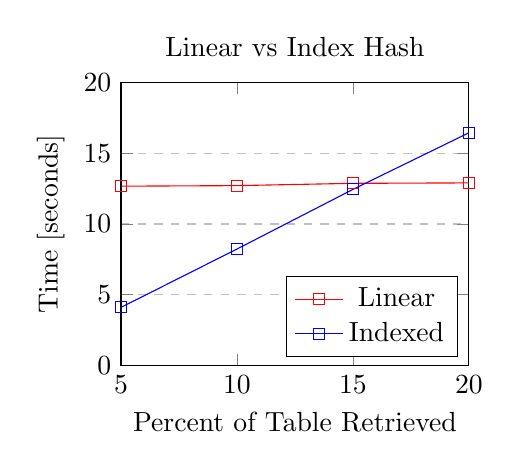
\begin{tikzpicture}
\begin{axis}[
    title={Linear vs Index Hash},
    xlabel={Percent of Table Retrieved},
    ylabel={Time [seconds]},
    xmin=5, xmax=20,
    ymin=0, ymax=20,
    xtick={5, 10, 15, 20},
    ytick={0,5,10,15,20},
    legend pos=south east,
    ymajorgrids=true,
    grid style=dashed,
    ]
    \addplot[
    color=red,
    mark=square,
    ]
    coordinates {
    (5,12.67146)(10,12.71014)(15,12.87276)(20,12.90335)
    };
    \addplot[
    color=blue,
    mark=square,
    ]
    coordinates {
    (5,4.10491)(10,8.22869)(15,12.44472)(20,16.44773)
    };
    \legend{Linear, Indexed}
\end{axis}
\end{tikzpicture}
&
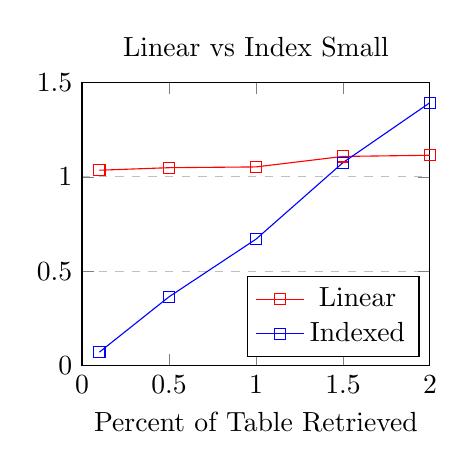
\begin{tikzpicture}
\begin{axis}[
    title={Linear vs Index Small},
    xlabel={Percent of Table Retrieved},
    %%ylabel={Time [seconds]},
    xmin=0, xmax=2,
    ymin=0, ymax=1.5,
    xtick={0,.5,1,1.5,2},
    ytick={0,.5,1,1.5},
    legend pos=south east,
    ymajorgrids=true,
    grid style=dashed,
    ]
    \addplot[
    color=red,
    mark=square,
    ]
    coordinates {
    (.1,1.035)(.5,1.04832)(1,1.05245)(1.5,1.10808)(2,1.11426)
    };
    \addplot[
    color=blue,
    mark=square,
    ]
    coordinates {
    (.1,.07065)(.5,.36386)(1,.66938)(1.5,1.07525)(2,1.39312)
    };
    \legend{Linear, Indexed}
\end{axis}
\end{tikzpicture}
&
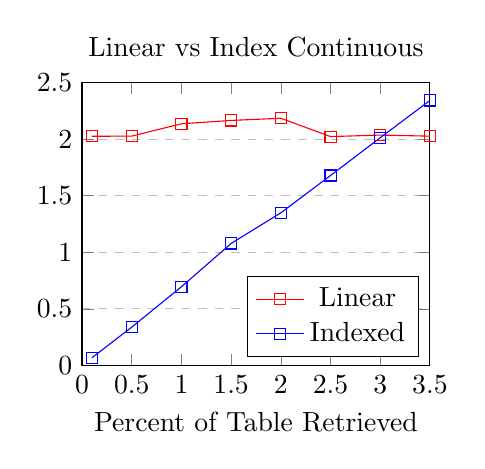
\begin{tikzpicture}
\begin{axis}[
    title={Linear vs Index Continuous},
    xlabel={Percent of Table Retrieved},
    %%ylabel={Time [seconds]},
    xmin=0, xmax=3.5,
    ymin=0, ymax=2.5,
    xtick={0,.5,1,1.5,2,2.5,3,3.5},
    ytick={0,.5,1,1.5,2,2.5},
    legend pos=south east,
    ymajorgrids=true,
    grid style=dashed,
    ]
    \addplot[
    color=red,
    mark=square,
    ]
    coordinates {
    (.1,2.02475)(.5,2.02638)(1,2.13519)(1.5,2.16479)(2,2.18408)(2.5,2.02196)(3,2.03547)(3.5,2.02588)
    };
    \addplot[
    color=blue,
    mark=square,
    ]
    coordinates {
    (.1,.06815)(.5,.33856)(1,.6951)(1.5,1.07784)(2,1.3485)(2.5,1.67818)(3,2.01217)(3.5, 2.34134)
    };
    \legend{Linear, Indexed}
\end{axis}
\end{tikzpicture}
\end{tabular}

\centering
\begin{tabular}{@{}l@{}l}
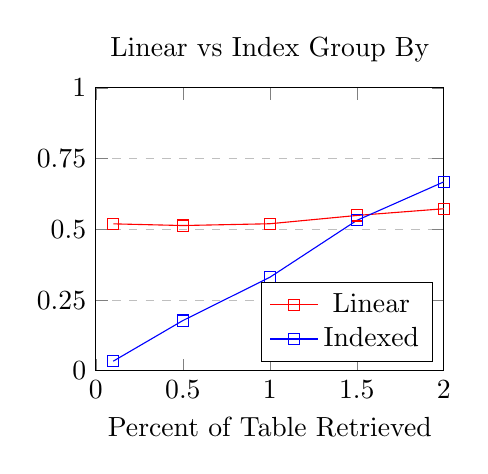
\begin{tikzpicture}
\begin{axis}[
    title={Linear vs Index Group By},
    xlabel={Percent of Table Retrieved},
    %%ylabel={Time [seconds]},
    xmin=0, xmax=2,
    ymin=0, ymax=1,
    xtick={0,.5,1,1.5,2},
    ytick={0,.25,.5,.75,1},
    legend pos=south east,
    ymajorgrids=true,
    grid style=dashed,
    ]
    \addplot[
    color=red,
    mark=square,
    ]
    coordinates {
    (.1,.51944)(.5,.51347)(1,.51979)(1.5,.54907)(2,.57281)
    };
    \addplot[
    color=blue,
    mark=square,
    ]
    coordinates {
    (.1,.03413)(.5,.17761)(1,.33048)(1.5,.53164)(2,.66775)
    };
    \legend{Linear, Indexed}
\end{axis}
\end{tikzpicture}
&
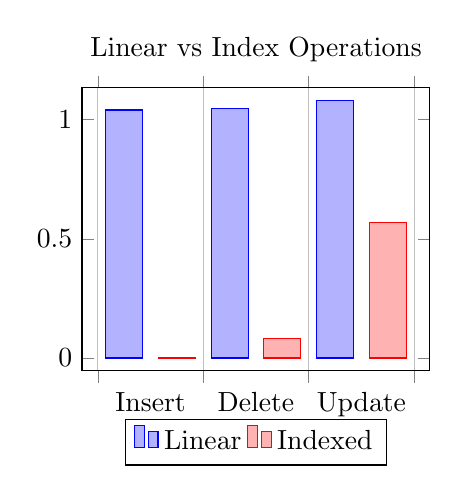
\begin{tikzpicture}
\begin{axis}[
    title={Linear vs Index Operations},
	symbolic x coords={Insert, Delete, Update, 4},
	x tick label style={
		/pgf/number format/1000 sep=},
	%%ylabel=Time (seconds),
	enlargelimits=0.05,
	legend style={at={(0.5,-0.17)},
	anchor=north,legend columns=-1},
	ybar interval=0.7,
    ]
\addplot 
	coordinates {(Insert,1.04077) (Delete,1.04533) (Update,1.0795) (4, 1)};
\addplot 
	coordinates {(Insert,.00024) (Delete,.08138) (Update,.57012) (4,1)};
    \legend{Linear, Indexed}
\end{axis}
\end{tikzpicture}\\
\end{tabular}
\caption{Comparison of Linear and Index versions of various operators. Linear scans do better when most of the data needs to be accessed regardless, but Indexed structures perform far better for small queries. Operations involving modification of the database are far faster for indexed structures.}
\label{figC1}
\end{figure*}

\begin{figure}
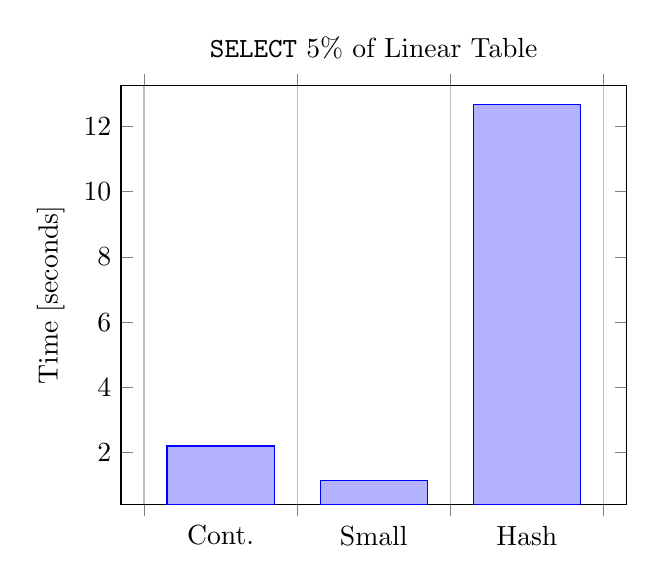
\begin{tikzpicture}
\begin{axis}[
	width=8cm,
	ylabel={Time [seconds]},
    title={\texttt{SELECT} 5\% of Linear Table}, 
	symbolic x coords={Cont., Small, Hash, 4},
	x tick label style={
		/pgf/number format/1000 sep=},
	%%ylabel=Time (seconds),
	enlargelimits=0.05,
	ybar interval=0.7,
    ]
\addplot 
	coordinates {(Cont., 2.20453) (Small, 1.14634) (Hash, 12.67146) (4, 1)};
\end{axis}
\end{tikzpicture}
\vskip 10pt
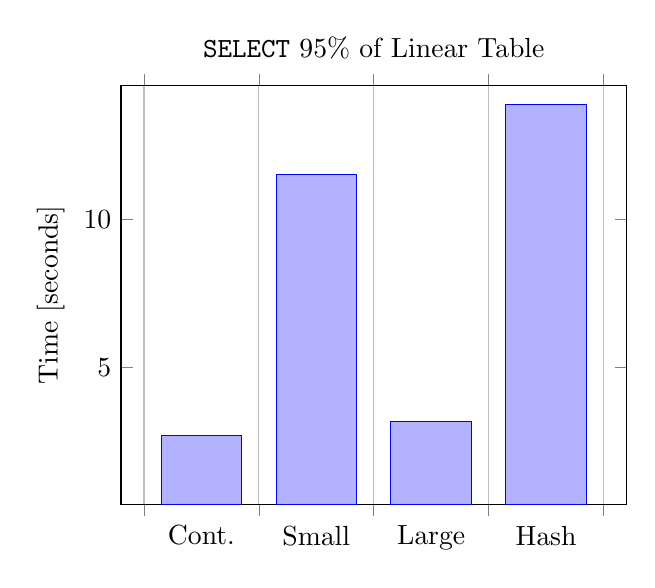
\begin{tikzpicture}
\begin{axis}[
	width=8cm,
	ylabel={Time [seconds]},
    title={\texttt{SELECT} 95\% of Linear Table},
	symbolic x coords={Cont., Small, Large, Hash, 4},
	x tick label style={
		/pgf/number format/1000 sep=},
	%%ylabel=Time (seconds),
	enlargelimits=0.05,
	ybar interval=0.7,
    ]
\addplot 
	coordinates {(Cont., 2.68609) (Small, 11.51625) (Large, 3.16022) (Hash, 13.89461) (4, 1)};
\end{axis}
\end{tikzpicture} 

\caption{Comparison of \texttt{SELECT} algorithms on Linear table where 5 and 95 percent of a table are retrieved. The Small and Large strategies do well in the 5\% and 95\% cases, respectively, and the Continuous strategy always performs well when applicable.} 
\label{figC3}
\end{figure}

\begin{figure*}
\begin{tabular}{@{}l@{}l@{}l}
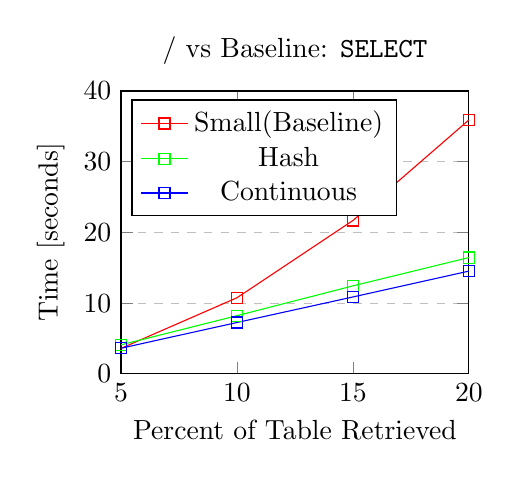
\begin{tikzpicture}
\begin{axis}[
    title={\name/ vs Baseline: \texttt{SELECT}},
    xlabel={Percent of Table Retrieved},
    ylabel={Time [seconds]},
    xmin=5, xmax=20,
    ymin=0, ymax=40,
    xtick={5, 10, 15, 20},
    ytick={0,10,20,30,40},
    legend pos=north west,
    ymajorgrids=true,
    grid style=dashed,
    ]
    \addplot[
    color=red,
    mark=square,
    ]
    coordinates {
    (5,3.60851)(10,10.76450)(15,21.68452)(20,35.90403)
    };
    \addplot[
    color=green,
    mark=square,
    ]
    coordinates {
    (5,4.10491)(10,8.22869)(15,12.44472)(20,16.44773)
    };
    \addplot[
    color=blue,
    mark=square,
    ]
    coordinates {
    (5,3.62659)(10,7.26511)(15,10.87671)(20,14.53167)
    };
    \legend{Small(Baseline), Hash, Continuous}
\end{axis}
\end{tikzpicture}
&
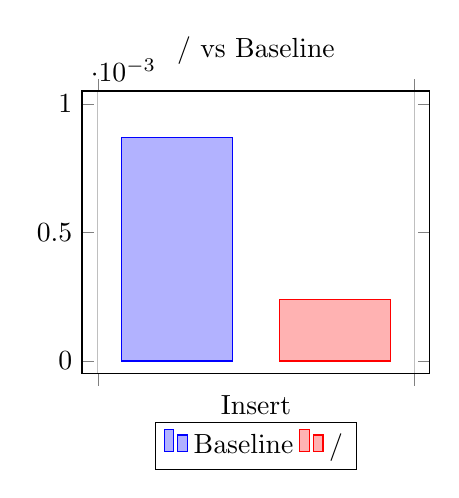
\begin{tikzpicture}
\begin{axis}[
    title={\name/ vs Baseline},
	symbolic x coords={Insert, 4},
	x tick label style={
		/pgf/number format/1000 sep=},
	%%ylabel=Time (seconds),
	enlargelimits=0.05,
	legend style={at={(0.5,-0.17)},
	anchor=north,legend columns=-1},
	ybar interval=0.7,
    ]
\addplot 
	coordinates {(Insert,.00087) (4, 0)};
\addplot 
	coordinates {(Insert,.00024) (4,.001)};
    \legend{Baseline, \name/}
\end{axis}
\end{tikzpicture}
&
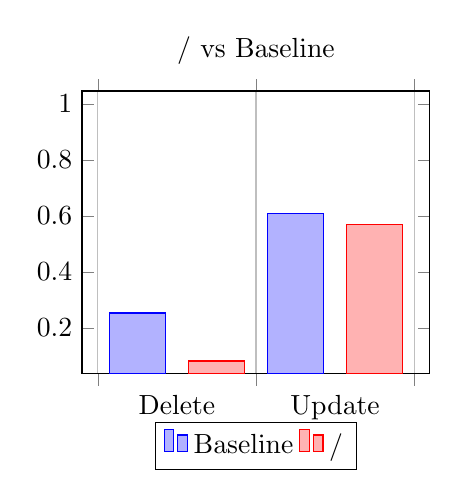
\begin{tikzpicture}
\begin{axis}[
    title={\name/ vs Baseline},
	symbolic x coords={Delete, Update, 4},
	x tick label style={
		/pgf/number format/1000 sep=},
	%%ylabel=Time (seconds),
	enlargelimits=0.05,
	legend style={at={(0.5,-0.17)},
	anchor=north,legend columns=-1},
	ybar interval=0.7,
    ]
\addplot 
	coordinates {(Delete,.25278) (Update,.60824) (4, 1)};
\addplot 
	coordinates {(Delete,.08138) (Update,.57012) (4,1)};
    \legend{Baseline, \name/}
\end{axis}
\end{tikzpicture}
\end{tabular}
\caption{Comparison between \name/ and a baseline solution where a B+ tree is generically ported to use ORAM and naive oblivious algorithms are used. \name/ significantly outperforms the baseline with its Hash and Continuous algorithms as well as its \texttt{Insert}, \texttt{Delete}, and \texttt{Update} operations.}
\label{figC2}
\end{figure*}

\begin{figure}
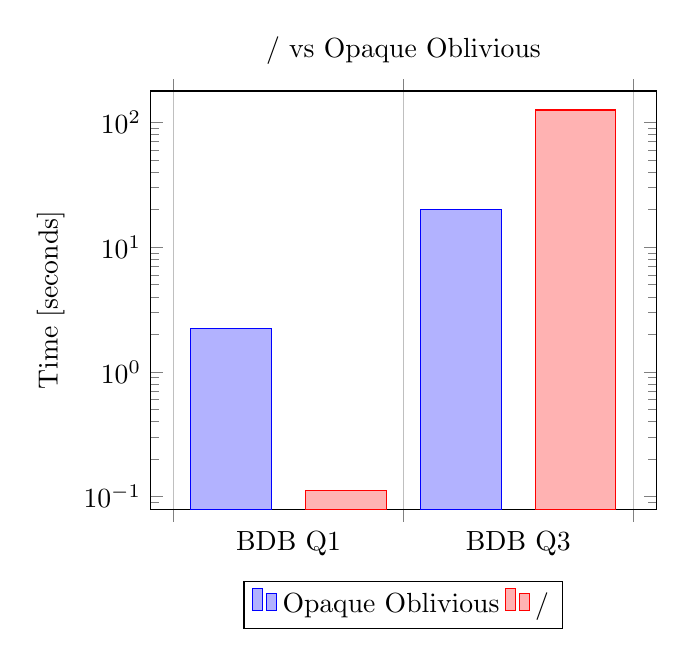
\begin{tikzpicture}
\begin{semilogyaxis}[
	log origin = infty,
	width=8cm,
	ylabel={Time [seconds]},
    title={\name/ vs Opaque Oblivious},
	symbolic x coords={BDB Q1, BDB Q3, 4},
	x tick label style={
		/pgf/number format/1000 sep=},
	%%ylabel=Time (seconds),
	enlargelimits=0.05,
	legend style={at={(0.5,-0.17)},
	anchor=north,legend columns=-1},
	ybar interval=0.7,
    ]
\addplot 
	coordinates {(BDB Q1,2.2437) (BDB Q3,19.9664) (4, 1)};
\addplot 
	coordinates {(BDB Q1,.11178) (BDB Q3,125.59) (4,1)};
    \legend{Opaque Oblivious, \name/}
\end{semilogyaxis}
\end{tikzpicture}
\caption{Comparison of \name/ and Opaque Oblivious mode on the Big data benchmark queries 1 and 3. \name/ outperforms Opaque on query 1 where it can leverage that advantage of its oblivious Indexed tables, but Opaque's custom-made oblivious analytics algorithms outperform \name/ when it uses a Linear table to compute the \texttt{INNER JOIN} in query 3.} 
\label{figOpaque}
\end{figure}
\name/ can handle real-world data sets with reasonable performance comparable to other solutions with more permissive leakage functions. We extensively evaluate \name/ on fabricated data with table sizes of up to 500,000 rows (results in the tables below are for tables of 100,000 rows) as well as three real data sets. NASDAQ \cite{NASDAQ} consists of the last sale price and other related information for all approximately 3200 stocks on the NASDAQ stock exchange. CFPB \cite{CFPB} contains individual complaints on financial products and services sent to the US consumer financial protection bureau and contains about 106,000 rows. Finally, FLIGHTS \cite{FLIGHT}, a subset of the flight dataset used to evaluate Splinter \cite{WYG+17}, contains data on arrival/departure points, flight numbers, ticket prices, and delays for 250,000 US domestic flights. A summary of queries executed on real-world data is shown in figure \ref{figQueries}. We also compare \name/ to prior work and show that it performs comparably or better. 

We will through our evaluation prove the following two claims: 

\begin{enumerate}
\item Choices of data structures and algorithms offered by \name/ allow for meaningful optimizations in handling queries without increasing leakage. 

\item \name/ performs better than a baseline solution that generically uses ORAM and comparably or better than prior work with similar or more permissive leakage.
\end{enumerate}

%paragraph summarizing evaluation results like in the introduction?

\subsection{Effectiveness of Low-Leakage Optimization}
We wish to show that providing both Indexed and Linear tables and optimizing \texttt{SELECT} queries based only on information from structureal leakage allows \name/ to make meaningful performance improvements for diverse data sets and queries. To this end, figure \ref{figC1} compares the performance of Linear and Indexed tables on various \texttt{SELECT} algorithms as well as \texttt{GROUP BY}, \texttt{INSERT}, \texttt{DELETE}, and \texttt{UPDATE} queries. Linear scans perform better as the amount of data retrieved from a table increases since the cost of the scan is amortized over more rows, but smaller queries perform significantly better using an index. Observe, moreover, in figure \ref{figQueries}, that queries perform better on Linear tables when the tables are smaller or involves aggregates over a whole table, but Indexed tables perform better when table sizes become large. This is not a surprising conclusion to draw, but it contrasts with claims in prior work \cite{RLT15} that claims linear scans perform better than ORAM for oblivious memory access. In general, Indexed \texttt{INSERT}, \texttt{DELETE}, and \texttt{UPDATE} queries significantly outperform Linear tables.

Figure \ref{figC3} demonstrates the effectiveness of \name/'s choice of \texttt{SELECT} algorithms, comparing our various algorithms on queries that retrieve 5\% and 95\% percent of a table. Although the ``Hash'' algorithm performs the best asymptotically, the figure demonstrates that knowledge gleaned only from \name/'s intended leakage about the results of a query (whether it is small, large, or a continuous set of rows) suffices to pick an algorithm that will perform dramatically better in practice. 

\subsection{Comparison to Baseline and Prior Work}

\name/'s Indexed tables perform better than a baseline implementation (e.g. what could be achieved with a generic tool for converting legacy applications). Figure \ref{figC2} shows comparisons between \name/ and a baseline solution where a database index is generically modified to provide obliviousness of data access patterns via an ORAM. Whereas \name/'s Indexed tables include a number of implementation optimizations to minimize the number of ORAM reads and writes needed in any query, our generic baseline makes an ORAM access every time a non-oblivious database would. The \texttt{INSERT} query is graphed separately because it runs much faster than \texttt{DELETE} and \texttt{UPDATE}. \texttt{INSERT} only needs to find one place in the tree to insert a row, whereas \texttt{DELETE} and \texttt{UPDATE} need to find a position in the leaves of the B+ tree and then scan forward until they find rows to update or delete. On average between the three operations, \name/ outperforms the baseline by approximately 70\%. 

The comparison of \texttt{SELECT} algorithms is complicated by the fact that a non-oblivious \texttt{SELECT}, if generically run over an ORAM, still leaks more than structural information when producing the Linear table that is returned to the user for display. We chose the naive ``Small'' strategy as a baseline because it is the most natural transformation of a non-oblivious \texttt{SELECT} to the oblivious setting. Although this baseline performs comparably to other strategies for queries with very small outputs, it rapidly falls behind the ``Hash'' and ``Continuous'' strategies as queries access more of the table. The figure shows this disparity reaching the point where \name/ outperforms the baseline by 60\% when a fifth of the table must be retrieved. 

\medskip \noindent \textbf{Comparison to Prior Work}\\

We compare \name/ to two recent works: the range search scheme of Demertzis et al \cite{DPP+16} and Opaque's Oblivious mode \cite{ZDB+17}. The range search scheme does not hide access patterns to data and lacks functionality for \texttt{JOIN}s. As we were not able to compare it directly to \name/, the best we can do is to examine the graphs in the original paper and observe that \name/'s performance is comparable or slightly better than that reported by \cite{DPP+16} on a similarly-sized USPS data set with more powerful hardware. 

Opaque, on the other hand, can be configured to provide the same security guarantees as \name/ in its OBLIV mode. The difference between Opaque and \name/ is that whereas Opaque is designed with data analytics in the distributed setting in mind and relies heavily on oblivious sorts, \name/ is developed as a standalone database system and makes use of ORAM to provide oblivious indexes. Figure \ref{figOpaque} compares the performance of \name/ and Opaque on queries 1 and 3 of the Big Data Benchmark \cite{BDB}. We were unable to compare \name/ and  Opaque on queries 2 and 4 of the benchmark because \name/'s high-cardinality aggregate algorithm is unimplemented (see Appendix \ref{groupby}) and neither system supports the external scripts needed for query 4. \name/ outperforms Opaque by 20x on query 1 and is 6.3x slower on query 3. The difference highlights the efficacy of \name/'s oblivious indexes, since query 1 is dramatically expedited by having an index that removes the requirement of examining all the data in order to fulfill the query. Query 3, on the other hand, involves an \texttt{INNER JOIN} that is executed over a Linear table in \name/, where Opaque's clever oblivious analytics algorithms give it the upper hand. We conclude from this that \name/ and Opaque are fundamentally well-suited to different kinds of problem domains, since \name/ excels when it can take advantages of its Indexed tables and Opaque performs well on queries that involve scanning over most or all of a table's contents. 


\section{Related Work}\label{related}

\name/ is related to a number of prior works involving cryptographically-protected databases and applications of trusted hardware.

\medskip \noindent \textbf{Cryptographically-protected database search}\\
A testament to the importance of the problem of search over encrypted data in databases lies in the extensive prior work on the subject, summarized and systematized by Fuller et al \cite{FVY+17}. Perhaps the most widely known work in this area is CryptDB \cite{PRZB12}, which implements a tradeoff between security and performance by encrypting each field in a table according to the type of operation expected to be used on the data in that field. Arx \cite{PBP16}, a more recent system, keeps all data encrypted at the highest level of security and makes clever use of data structures to allow for efficient operations over data. Another common class of solutions are those which use an inverted index to allow searches on stored encrypted data, as exemplified by Demertzis et al \cite{DPP+16}. These schemes rely on searchable symmetric encryption (SSE) as a primitive, a recent example of which is Sophos \cite{Bost16}, which boasts forward security in the sense that queries authorized in the past do not leak any new information when additional documents are added to an existing database. 

The diversity of security goals and varied use cases for which cryptographically protected databases have been designed have led to a plague of attacks which show that real-world applications of schemes proven secure in theoretical models can in fact leak far more data than would be expected from an initial examination of a system's security properties. Initiated by Islam et al \cite{IKK12} and continuing with improved results such as those of Naveed et al \cite{NKW15} and Cash et al \cite{CGPR15} to name only a few, such attacks show that inference from known context of the data used, additional correlated public data, or even just the leakage inherent in a scheme itself, can be used to attack various schemes in ways not anticipated in their original security models. Zhang et al \cite{ZKP16} show that even schemes with very little leakage are susceptible to attack. In hiding even the access patterns to data in our solution, we hope to minimize the extent to which \name/ is vulnerable to such techniques.   

\medskip \noindent \textbf{Trusted hardware}\\
Trusted hardware can be used to achieve security properties that are difficult, impractical, or potentially impossible with traditional cryptographic assumptions. For example, a number of hardware or hardware/software based solutions exist with the explicit goal of rendering programs' memory traces oblivious \cite{CLD16, LHM+15, MLS+13}. Intel SGX, on which we will focus, has in particular been used to implement practical functional encryption \cite{FVBG16} and obfuscation \cite{NFR+17}, both functionalities which can currently only be constructed using heavy cryptographic machinery.

In recent years, a number of generic tools have been designed to provide legacy applications the heightened security available from SGX. Haven \cite{BPH15} shields execution of legacy programs from a malicious OS. Panoply and SCONE \cite{STTS17, ATG+16} provide SGX-protected Linux operating system and container abstractions. In the distributed setting, Ryoan \cite{HZX+16} is a sandbox for computation on secret data. 

In addition to general tools, applications to securely conduct data analytics or handle data in the cloud represent a compelling practical use case for SGX hardware. In this vein, many works implement variations of existing tools and services rendered secure via SGX. M2R \cite{DSC+15} and VC3 \cite{SCF+15} provide MapReduce and cloud data analytics functionalities, respectively, and Opaque \cite{ZDB+17} provides secure support for Spark SQL. SecureKeeper \cite{BWG+16} uses SGX to build a confidential version of Apache's ZooKeeper (\url{zookeeper.apache.org}). More fundamental primitives for databases and oblivious computation in general are provided by HardIDX \cite{FBB+17}, a database index in SGX, and ZeroTrace \cite{SGF17} which provides oblivious memory primitives based on ORAM as well as an analysis of parameter optimizations for using an ORAM controller in SGX for data storage. None of the solutions above, with the exception of ZeroTrace, use ORAM to hide memory access patterns. Instead, they either make use of memory-oblivious algorithms suited to the tasks they undertake or remain vulnerable to side-channel attacks targeting memory access patterns. 

Trusted hardware assumption like those underlying the use of SGX as a secure platform fundamentally differ from traditional mathematical assumptions in that, whereas the validity of a mathematical assumption cannot be challenged by the vicissitudes of succeeding implementations, attacks, and side-channels, the legitimacy of a hardware assumption relies directly on the ability of a piece of manufactured hardware to repel practical attacks. As such, the SGX literature includes a number of works that aim to reveal practical side channels in the implementation of SGX and develop techniques to obviate the risks presented by each known family of attacks. Xu et al \cite{XCP15} use page faults and other ``controlled channel'' side channels to extract images and text documents from protected memory, and Lee et al \cite{LSG+16} use the fact that SGX does not clear branch history when leaving an enclave to infer details of branches taken in protected code. In the multithreaded regime, Weichbrodt et al \cite{WKPK16} compromise security by leveraging synchronization bugs. Defenses against such attacks include the work of Shinde et al \cite{SCNS16} and Raccoon \cite{RLT15} which close side channels by making the memory trace of a program oblivious or obfuscated. SGX-Shield \cite{SLK+17} enables address space layout randomization for SGX, and, finally, T-SGX \cite{SLKP17} protects against side-channel attacks by using another set of hardware features, Transactional Synchronization Extensions (TSX) to close side channels that could otherwise be exploited by a malicious operating system. \name/ can be generically combined with any of these solutions to provide higher levels of confidence in the security of the enclave. 

\section{Conclusion}\label{conclusion}
We have presented \name/, a cryptographically-protected database system based on Intel SGX with little to no leakage beyond structural information about data and responses to queries. We have shown that \name/ handles practical data sets with acceptable performance comparable to other existing solutions with more permissive leakage functions. It is our hope that solutions like \name/ based on SGX and other techniques that leverage hardware-based advantages can enable rapid advances in the performance and security of solutions to difficult problems related to private databases and search over encrypted data. 

\section*{Acknowledgements}



\bibliographystyle{plain}
\bibliography{oramsgx}

\appendix

\section{Support for Unbounded Numbers of Groups}\label{groupby}
As mentioned in section \ref{oblivOps}, our implementation of \name/ supports a large but fixed maximum number of groups. Here we mention ideas that could be implemented to increase this limit to support arbitrary high-cardinality aggregation. 

First, if the number of groups is larger than can be kept in the enclave at once, it becomes important to be able to count the total number on a first pass. This can be accomplished with the HyperLogLog algorithm \cite{FFGM07}. Once this is done, it is possible to make multiple passes over the table being selected from, each time calculating the aggregate for as many groups as possible. In order to make sure each group is aggregated only once, each pass will cover successive groups in alphabetical order and the enclave will store the name of the last alphabetical group to have been aggregated. To make sure each pass only aggregates groups in alphabetical order, the algorithm will hae to check on each row whether the group to which the row belongs is alphabetically prior to any group permanently being aggregated. If so, that row is given a place in the enclave and the alphabetically last group under consideration is thrown out to be re-examined on a future pass. 

If the number of groups were large enough that the above solution becomes impractical because it requires a number of passes linear in the number of groups, another solution would be to, after completing the HyperLogLog scan, create a copy of the table $T$ called $T'$ and sort it obliviously by group. Then, after creating $O$ of size $o$ as determined by the HyperLogLog algorithm, one additional scan over the sorted table could be done, with the aggregate value for each group being calculated as that group is reached in $T'$. 
\end{document}
